\documentclass[preprint,12pt,aps,pra,showkeys,amsmath,amssymb,superscriptaddress,floatfix]{revtex4-2}
\usepackage[T1]{fontenc}
\usepackage[utf8]{inputenc}
\usepackage{amsmath,amssymb,amsthm,mathtools,mathrsfs}
\usepackage{microtype,booktabs,enumitem}
\usepackage{xcolor,tikz,etoolbox}
\usepackage[skins,breakable]{tcolorbox}
\usepackage{needspace}
% Keep diagram geometry independent of REVTeX preprint body spacing.
\AtBeginEnvironment{tikzpicture}{\linespread{1}\selectfont}
\usetikzlibrary{arrows.meta,positioning,calc,fit,decorations.pathreplacing}
\usepackage{graphicx}
\usepackage{hyperref}

\definecolor{MMBlue}{RGB}{0,82,155}
\definecolor{MMOrange}{RGB}{200,80,0}
\tikzset{
 mmnode/.style={draw=MMBlue,rounded corners=2pt,fill=MMBlue!4,align=left,execute at begin node={\raggedright},text width=5cm,font=\fontsize{10}{12}\selectfont,inner sep=6pt},
 mmimport/.style={mmnode,draw=black!65,fill=black!4},
 mmcandidate/.style={mmnode,draw=MMOrange,dashed,fill=MMOrange!5},
 mmrejected/.style={mmnode,draw=black,densely dotted,fill=black!8},
 mmproof/.style={->,thick,MMBlue},
 mmflow/.style={->,semithick,black!70},
 mmrepair/.style={->,dashed,thick,MMOrange},
 mmcandidatearrow/.style={->,dashed,semithick,MMOrange},
 mmnote/.style={font=\scriptsize,fill=white,inner sep=2pt,align=center}}

\usepackage[section]{placeins}
\setlength{\emergencystretch}{3em}
\setlist{itemsep=3pt,topsep=4pt}
\newtheorem{theorem}{Theorem}[section]
\newtheorem{proposition}[theorem]{Proposition}
\newtheorem{lemma}[theorem]{Lemma}
\newtheorem{corollary}[theorem]{Corollary}
\theoremstyle{definition}
\newtheorem{definition}[theorem]{Definition}
\newtheorem{example}[theorem]{Example}
\theoremstyle{remark}
\newtheorem{remark}[theorem]{Remark}
% Avoid isolated statement headings and single-line paragraph fragments.
\BeforeBeginEnvironment{theorem}{\Needspace{6\baselineskip}}
\BeforeBeginEnvironment{definition}{\Needspace{5\baselineskip}}
\BeforeBeginEnvironment{proposition}{\Needspace{5\baselineskip}}
\BeforeBeginEnvironment{lemma}{\Needspace{5\baselineskip}}
\BeforeBeginEnvironment{corollary}{\Needspace{5\baselineskip}}
\clubpenalty=5000
\widowpenalty=5000
\newcommand{\R}{\mathbb R}\newcommand{\Z}{\mathbb Z}\newcommand{\N}{\mathbb N}
\newcommand{\Pa}{\operatorname{Pa}}\newcommand{\Desc}{\operatorname{Desc}}
\newcommand{\cl}{\operatorname{cl}}\newcommand{\cost}{\operatorname{cost}}
\newcommand{\status}{\operatorname{status}}
% Faculty cards: a visual rail groups the five faculties within one agent.
% The rail has no arrowhead and does not represent a proof dependency.
\newcommand{\mmfacultybadge}[1]{%
 \node[circle,draw=MMBlue,line width=1pt,fill=white,
 minimum size=7mm,inner sep=0pt,font=\sffamily\small\bfseries,text=MMBlue]
 at ([xshift=15pt,yshift=-15pt]frame.north west) {#1};}
\newcommand{\mmfacultyrail}{%
 \draw[MMBlue!80,line width=1pt]
 ([xshift=15pt,yshift=2pt]frame.north west)--
 ([xshift=15pt,yshift=-2pt]frame.south west);}
\newtcolorbox{mmfacultybox}[2]{enhanced,breakable,
 colback=MMBlue!4,colframe=MMBlue!4,boxrule=0pt,arc=3pt,
 left=39pt,right=9pt,top=4pt,bottom=4pt,
 before skip=2pt,after skip=2pt,
 fontupper=\small\linespread{1.1}\selectfont,
 overlay unbroken={\mmfacultyrail\mmfacultybadge{#1}},
 overlay first={\mmfacultyrail\mmfacultybadge{#1}},
 overlay middle={\mmfacultyrail},overlay last={\mmfacultyrail}}
\newcommand{\mmfaculty}[3]{%
 \begin{mmfacultybox}{#1}{#2}
 {\sffamily\bfseries\color{MMBlue}#2}\par\smallskip #3
 \end{mmfacultybox}}
\newcommand{\agent}[9]{%
 \Needspace{8\baselineskip}
 \subsubsection{#1}
 \noindent\textbf{Object.} #2\par
 \noindent\textbf{Role.} #3\par\smallskip
 \mmfaculty{E}{Ego}{#4}
 \mmfaculty{M}{Memory}{#5}
 \mmfaculty{I}{Intellect}{#6}
 \mmfaculty{S}{Sense}{#7}
 \mmfaculty{A}{Action}{#8}
 \smallskip\noindent #9\par}

\usepackage{longtable,array,calc}
\providecommand{\tightlist}{\setlength{\itemsep}{2pt}\setlength{\parskip}{0pt}}
\makeatletter
\def\frontmatter@abstract@produce{\par\addvspace{\frontmatter@preabstractspace}%
\begingroup\prep@absbox\unvbox\absbox\post@absbox\endgroup
\addvspace{\frontmatter@postabstractspace}}
\makeatother
\newcommand{\field}[2]{\par\smallskip\noindent\textbf{#1.} #2\par}
\setlength{\emergencystretch}{5em}
\AtBeginEnvironment{verbatim}{\small\linespread{1.0}\selectfont}


\hypersetup{colorlinks=true,linkcolor=MMBlue,urlcolor=MMBlue,pdfauthor={Dibakar Sigdel}}

\begin{document}

\title{Undecidability of the Halting Problem\\[4pt]\large An End-to-End Meta-Math Walkthrough}

\author{Dibakar Sigdel}

\affiliation{Mindverse Computing LLC, Lynnwood, WA 98087, USA}

\date{October 2026}

\begin{abstract}

Assuming a decider allows construction of a machine that reverses its
answer on the diagonal input. The contradiction concerns a total
decision procedure; direct simulation still provides a one-sided
recognition procedure. The report presents the target theorem, declared
imports, a dependency graph, five-faculty node contracts, a continuous
proof, a worked example, and a hypothesis-repair audit. It is an
authored mathematical exposition, not a deployed-agent transcript or a
formal proof-assistant certificate.

\end{abstract}\maketitle\linespread{1.12}\selectfont

\noindent\textbf{LF-05 / Mathematical Logic and Set Theory / Report v1}

\section{Target and import contract}

\begin{theorem}

Fix an effective encoding of deterministic Turing machines by finite
strings. Prove no total computable function \(H(e,x)\in\{0,1\}\)
correctly decides for every valid machine code \(e\) and input string
\(x\) whether that machine eventually halts on \(x\). Also prove the
halting set is computably enumerable: there is a procedure that halts
and accepts exactly the halting pairs. Invalid codes can be assigned a
fixed decidable convention and do not affect the result.

\end{theorem}

\subsection{Foundations and permitted imports}

Use a universal step-by-step simulator for the fixed Turing-machine
model, effective composition and conditional branching of finite
programs, and the ability to implement an infinite loop. Every such
finite program has an encoding in the same model. These are elementary
properties of the computational model, not an oracle or a solution of
the target decision problem.

\clearpage\section{Node interaction workflow}

\begin{center}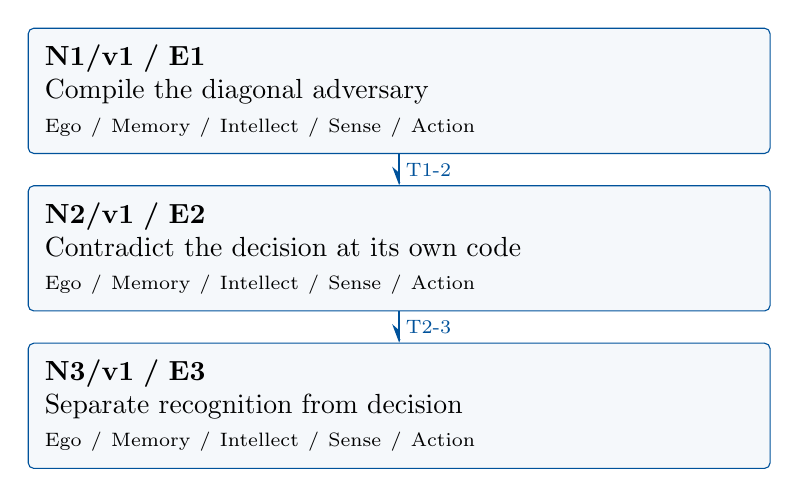
\begin{tikzpicture}[>=Stealth,x=1cm,y=1cm]

\node[mmnode,text width=9cm,minimum height=1.25cm] (N1) at (0,0.0) {\textbf{N1/v1 / E1}\\Compile the diagonal adversary\\{\scriptsize Ego / Memory / Intellect / Sense / Action}};

\node[mmnode,text width=9cm,minimum height=1.25cm] (N2) at (0,-2.0) {\textbf{N2/v1 / E2}\\Contradict the decision at its own code\\{\scriptsize Ego / Memory / Intellect / Sense / Action}};

\node[mmnode,text width=9cm,minimum height=1.25cm] (N3) at (0,-4.0) {\textbf{N3/v1 / E3}\\Separate recognition from decision\\{\scriptsize Ego / Memory / Intellect / Sense / Action}};

\draw[mmproof] (N1.south) -- node[mmnote,right] {T1-2} (N2.north);

\draw[mmproof] (N2.south) -- node[mmnote,right] {T2-3} (N3.north);

\end{tikzpicture}\end{center}

Each box is one mathematical agent containing all five faculties. Blue
arrows carry the versioned exports listed below. The layout gives a
reading order; only drawn arrows assert dependencies. Diagnostic repair
is separate from the proof DAG.

\subsection{Versioned evidence-transfer ledger}

\begingroup\small\linespread{1.05}\selectfont

\Needspace{5\baselineskip}\field{T1-2: N1/E1/v1 to N2}{There is a machine \(D\) with a valid code \(d\) such that \(D(z)\)
loops if \(H(z,z)=1\) and halts if \(H(z,z)=0\).}

\field{Receiving activity}{N2.1}

\field{Compatibility}{E1/v1 and the purported correctness of \(H\) on the valid pair
\((d,d)\). Check: The contradiction is to the existence of a correct
total \(H\), not to the existence of the perfectly valid looping machine
\(D\).}

\Needspace{5\baselineskip}\field{T2-3: N2/E2/v1 to N3}{No total computable halting decider exists.}

\field{Receiving activity}{N3.2}

\field{Compatibility}{A valid encoded machine-input pair and the universal simulator; E2/v1
for the distinction from decision. Check: Failure to observe a halt by a
finite time does not certify nonhalting.}

\endgroup

\clearpage\section{Agent roles and five-faculty activities}\begingroup\small\linespread{1.05}\selectfont\setlist{itemsep=1pt,topsep=2pt}

\subsection{N1/v1: Compile the diagonal adversary}

\field{Object and role}{Construct a finite machine that consults \(H(z,z)\) and then
deliberately does the opposite. \textbf{Local obligation:} There is a
machine \(D\) with a valid code \(d\) such that \(D(z)\) loops if
\(H(z,z)=1\) and halts if \(H(z,z)=0\).}

\field{Inputs}{A hypothetical total computable correct decider \(H\).}

\mmfaculty{E}{Ego}{Publish E1/v1 only after establishing this obligation: There is a
machine \(D\) with a valid code \(d\) such that \(D(z)\) loops if
\(H(z,z)=1\) and halts if \(H(z,z)=0\).}

\mmfaculty{M}{Memory}{A hypothetical total computable correct decider \(H\). Retain the stated
assumptions and import versions.}

\mmfaculty{I}{Intellect}{Construct a finite machine that consults \(H(z,z)\) and then
deliberately does the opposite.}

\mmfaculty{S}{Sense}{Totality makes the branch selection terminate; the constructed machine
may itself loop, which is permitted for an ordinary machine.}

\mmfaculty{A}{Action}{Carry out activities N1.1--N1.2 below, retaining each calculation and
construction as evidence.}

\smallskip\noindent\textbf{Numbered mathematical activities}

\begin{enumerate}[label=N1.\arabic*,leftmargin=3.4em]

\item Define a program on input \(z\): compute \(H(z,z)\); if the result is
one, execute an infinite loop; if the result is zero, halt. Under the
hypothesis, the computation of \(H\) always finishes and this is an
effective finite program.

\item By the fixed model's effective composition and encoding, this program is
a Turing machine with some valid code \(d\). Giving a program its own
code as an input is legal: codes are finite strings and machines accept
finite strings. No machine needs to discover its own code internally.

\end{enumerate}

\field{Export E1/v1}{There is a machine \(D\) with a valid code \(d\) such that \(D(z)\)
loops if \(H(z,z)=1\) and halts if \(H(z,z)=0\).}

\field{Acceptance gate}{Totality makes the branch selection terminate; the constructed machine
may itself loop, which is permitted for an ordinary machine.}

\field{Targeted repair}{If the argument assumes a possibly nonterminating test before branching,
restore the total-decider hypothesis; without it the reversal would not
be implemented on every input. Withhold this export and recheck its
descendants after a versioned correction.}

\clearpage

\subsection{N2/v1: Contradict the decision at its own code}

\field{Object and role}{Exhaust both possible Boolean answers and compare them with the
constructed behavior. \textbf{Local obligation:} No total computable
halting decider exists.}

\field{Inputs}{E1/v1 and the purported correctness of \(H\) on the valid pair
\((d,d)\). Incoming proof exports: E1/v1 at N2.1.}

\mmfaculty{E}{Ego}{Publish E2/v1 only after establishing this obligation: No total
computable halting decider exists.}

\mmfaculty{M}{Memory}{E1/v1 and the purported correctness of \(H\) on the valid pair
\((d,d)\). Incoming proof exports: E1/v1 at N2.1. Retain the stated
assumptions and import versions.}

\mmfaculty{I}{Intellect}{Exhaust both possible Boolean answers and compare them with the
constructed behavior.}

\mmfaculty{S}{Sense}{The contradiction is to the existence of a correct total \(H\), not to
the existence of the perfectly valid looping machine \(D\).}

\mmfaculty{A}{Action}{Carry out activities N2.1--N2.2 below, retaining each calculation and
construction as evidence.}

\smallskip\noindent\textbf{Numbered mathematical activities}

\begin{enumerate}[label=N2.\arabic*,leftmargin=3.4em]

\item If \(H(d,d)=1\), correctness predicts that \(D(d)\) halts. But by
construction that branch loops forever, a contradiction.

\item If \(H(d,d)=0\), correctness predicts that \(D(d)\) never halts. But the
other branch halts immediately after the completed call to \(H\), also a
contradiction. These exhaust the two outputs, so the supposed decider
cannot exist.

\end{enumerate}

\field{Export E2/v1}{No total computable halting decider exists.}

\field{Acceptance gate}{The contradiction is to the existence of a correct total \(H\), not to
the existence of the perfectly valid looping machine \(D\).}

\field{Targeted repair}{If only one answer branch is analyzed, check the other explicitly;
undecidability requires defeating every possible returned answer.
Withhold this export and recheck its descendants after a versioned
correction.}

\clearpage

\subsection{N3/v1: Separate recognition from decision}

\field{Object and role}{Simulate one step at a time and accept when a halt is observed.
\textbf{Local obligation:} The halting set is computably enumerable but
not decidable.}

\field{Inputs}{A valid encoded machine-input pair and the universal simulator; E2/v1
for the distinction from decision. Incoming proof exports: E2/v1 at
N3.2.}

\mmfaculty{E}{Ego}{Publish E3/v1 only after establishing this obligation: The halting set
is computably enumerable but not decidable.}

\mmfaculty{M}{Memory}{A valid encoded machine-input pair and the universal simulator; E2/v1
for the distinction from decision. Incoming proof exports: E2/v1 at
N3.2. Retain the stated assumptions and import versions.}

\mmfaculty{I}{Intellect}{Simulate one step at a time and accept when a halt is observed.}

\mmfaculty{S}{Sense}{Failure to observe a halt by a finite time does not certify nonhalting.}

\mmfaculty{A}{Action}{Carry out activities N3.1--N3.2 below, retaining each calculation and
construction as evidence.}

\smallskip\noindent\textbf{Numbered mathematical activities}

\begin{enumerate}[label=N3.\arabic*,leftmargin=3.4em]

\item On input \((e,x)\), simulate the machine coded by \(e\) on \(x\) one
step at a time. If the simulated machine reaches a halting state,
accept. If it never halts, the simulator continues forever. Thus the
procedure accepts exactly the halting pairs.

\item This is a recognizer, not a decider, because nonhalting inputs need not
return an answer. In conjunction with E2, it proves that the halting set
is computably enumerable and undecidable.

\end{enumerate}

\field{Export E3/v1}{The halting set is computably enumerable but not decidable.}

\field{Acceptance gate}{Failure to observe a halt by a finite time does not certify nonhalting.}

\field{Targeted repair}{If simulation is presented as a decision procedure, state its
nonterminating behavior on negative instances and keep the
recognition/decision distinction. Withhold this export and recheck its
descendants after a versioned correction.}

\endgroup\clearpage\section{Continuous mathematical proof}\label{sec:proof}

\subsection{N1 --- Compile the diagonal
adversary}\label{n1-compile-the-diagonal-adversary}

\begin{enumerate}
\def\labelenumi{\arabic{enumi}.}
\item
  \textbf{N1.1.} Define a program on input \(z\): compute \(H(z,z)\); if
  the result is one, execute an infinite loop; if the result is zero,
  halt. Under the hypothesis, the computation of \(H\) always finishes
  and this is an effective finite program.
\item
  \textbf{N1.2.} By the fixed model's effective composition and
  encoding, this program is a Turing machine with some valid code \(d\).
  Giving a program its own code as an input is legal: codes are finite
  strings and machines accept finite strings. No machine needs to
  discover its own code internally.
\end{enumerate}

\subsection{N2 --- Contradict the decision at its own
code}\label{n2-contradict-the-decision-at-its-own-code}

\begin{enumerate}
\def\labelenumi{\arabic{enumi}.}
\item
  \textbf{N2.1.} If \(H(d,d)=1\), correctness predicts that \(D(d)\)
  halts. But by construction that branch loops forever, a contradiction.
\item
  \textbf{N2.2.} If \(H(d,d)=0\), correctness predicts that \(D(d)\)
  never halts. But the other branch halts immediately after the
  completed call to \(H\), also a contradiction. These exhaust the two
  outputs, so the supposed decider cannot exist.
\end{enumerate}

\subsection{N3 --- Separate recognition from
decision}\label{n3-separate-recognition-from-decision}

\begin{enumerate}
\def\labelenumi{\arabic{enumi}.}
\item
  \textbf{N3.1.} On input \((e,x)\), simulate the machine coded by \(e\)
  on \(x\) one step at a time. If the simulated machine reaches a
  halting state, accept. If it never halts, the simulator continues
  forever. Thus the procedure accepts exactly the halting pairs.
\item
  \textbf{N3.2.} This is a recognizer, not a decider, because nonhalting
  inputs need not return an answer. In conjunction with E2, it proves
  that the halting set is computably enumerable and undecidable.
\end{enumerate}

\hfill$\square$

\section{Worked orchestration}

A machine that immediately halts on any input is accepted by the
simulator after finitely many steps. A machine with a single transition
back to the same nonhalting state is simulated indefinitely. If a
hypothetical decider labels the diagonal machine \(D(d)\) as halting,
its prescribed branch is the loop; if it labels it nonhalting, its
branch halts. The contradiction is symbolic and does not claim that such
a decider was run.

\subsection{Boundary and hypothesis audit}

The theorem does not say no individual nonhalting behavior can be
proved. The one-state self-loop is easy to certify, and any fixed finite
collection of known examples can be classified. What is impossible is
one total computable procedure that is correct on every machine-input
pair in the stated unbounded model.

\section{Illustrative failure and repair}

The following is an authored diagnostic scenario. Changed assumptions
define a new contract; they do not retroactively prove the original
statement.

\subsection{Rejected argument, diagnosis, and correction}
\textbf{Rejected N3 rule:} after a million simulated steps without
halting, return ``never halts.'' A finite program can count to a million
plus one and then halt. \textbf{Diagnosis:} Sense identifies finite
observation being promoted to an unbounded universal claim.
\textbf{Repair:} let the recognizer keep running on unresolved inputs;
it remains a valid semidecision procedure but no longer claims totality.
This is an explicit weakening of the rejected algorithmic claim,
consistent with the proved impossibility theorem.

\subsection{Publication and reuse}
The corrected export retains its explicit assumptions. A hypothetical
revision receives a new version, and each consuming activity is
rechecked; this scenario is not a recorded runtime event. \textbf{Next
direction:} Develop many-one reductions to transfer undecidability to
other decision problems, recording the computability and correctness of
each reduction.

\par\medskip\begingroup\small\linespread{1.0}\selectfont\noindent\textbf{Provenance.} This authored proof is complete relative to its declared imports. Reuse
each export with its assumptions, proof, and version. The original
Markdown remains available for comparison.
\par\endgroup

\par\smallskip\begingroup\small\linespread{1.0}\selectfont\noindent\textbf{Further reading.} \href{https://math.berkeley.edu/~marks/notes/set_theory_notes_4.pdf}{Andrew
Marks, Set Theory notes} for sets and ultraproducts;
\href{https://math.berkeley.edu/~antonio/math125A/mathlogicP1.pdf}{Berkeley,
Mathematical Logic for Mathematicians, Part I} for first-order
semantics;
\href{https://math.berkeley.edu/~marks/notes/computability_notes_v1.pdf}{Andrew
Marks, Computability Theory notes} for effective procedures and
undecidability. The proofs below specify their own set-theoretic and
semantic assumptions.\par\endgroup

\end{document}
